\documentclass[a4paper]{article}
\def\DOCTITLE{CSC3621 Cryptography}
% Set document attributes
\title{\DOCTITLE}

\usepackage{fullpage}
\usepackage{scrextend}
\usepackage{titlesec}
\usepackage{fancyhdr}
\usepackage{amsmath}
\usepackage{amssymb}

% Handle graphics correctly
\ifx\pdftexversion\undefined
\usepackage{graphicx}
% \usepackage[dvips]{graphicx}
\else
\usepackage[pdftex]{graphicx}
\DeclareGraphicsRule{*}{mps}{*}{}
\fi

% Setup headers and footers
\pagestyle{fancy}
\lhead{}
\chead{\DOCTITLE}
\rhead{}
\rfoot{}
\cfoot{\thepage}
\lfoot{}

% New page for each section
% \newcommand{\sectionbreak}{\clearpage}

% Set header and footer sizes
\renewcommand{\headrulewidth}{0.4pt}
\renewcommand{\footrulewidth}{0.4pt}
\setlength{\headheight}{15.2pt}
\setlength{\headsep}{15.2pt}

\setlength{\parskip}{5pt plus 1pt minus 1pt}
\setlength{\parindent}{0pt}

\newcommand{\Forall}{\;\forall\;}
\newcommand{\Mod}{\: mod \:}


\begin{document}

\tableofcontents

\section{Maths}

\subsection{Discrete Probability}

Given a finite sample space $S = \{s_{1}, s_{2}, \ldots, s_{n}\}$ the probability
$P$ on $S$ is $\{p_{1}, p_{2}, \ldots,p_{n}\}$ where:

\begin{align*}
  0 \leq p_{i} \leq 1 \\
  \sum_{i}p_{i} = 1
\end{align*}

\subsubsection{Events}

\begin{itemize}
  \item Event $E$ is a subset of $S$
  \item Complimentary event $\bar{E}$
  \item Probability of occurrence $P(E)$
  \item $P(E) = 1 - P(\bar{E})$
\end{itemize}

\subsubsection{Joint Probability}

\begin{itemize}
  \item Probability of both events occurring
  \item $P(E_{1} \cap E_{2})$
  \item Events $E_{1}$ and $E_{2}$ are mutually exclusive if $P(E_{1} \cap
        E_{2}) = 0$
\end{itemize}

\subsubsection{Conditional Probability}

Assuming $P(E_{2}) > 0$.

Probability of $E_{1}$ happening given that $E_{2}$ has happened:
\[
  P(E_{1} | E_{2}) = \frac{P(E_{1} \cap E_{2})}
                          {P(E_{2})}
\]

$E_{1}$ and $E_{2}$ are independent if $P(E_{1} | E_{2}) = P(E_{1})P(E_{2})$.

\subsubsection{Bayes Theorem}

Assuming $P(E_{2}) > 0$.

\[
  P(E_{1} | E_{2}) = \frac{P(E_{1})P(E_{2} | E_{1})}
                          {P(E_{2})}
\]

\subsection{Complexity}

\begin{description}
  \item[Polynomial time] \hfill \\
    Solved in $O(n^{k})$
  \item[Exponential time] \hfill \\
    Cannot be solved in polynomial time
\end{description}

Decision problems that can be solved in polynomial time are tractable, otherwise
they are intractable.

\subsubsection{Complexity classes}

\begin{description}
  \item[P] \hfill \\
    Can be solved in polynomial time
  \item[NP] \hfill \\
    A positive answer can be verified in polynomial time
  \item[co-NP] \hfill \\
    A negative answer can be verified in polynomial time
  \item[NP-complete] \hfill \\
    Hardest problems in NP
\end{description}

\begin{figure}[h!]
  \centering
  
\includegraphics[width=0.5\textwidth]{out/complexity_classes.eps}
  \caption{Complexity Classes}
  \label{fig:complexity_classes}
\end{figure}
\FloatBarrier

\subsection{Number Theory}

\begin{itemize}
  \item $\mathbb{N}$ denotes positive integer such that $N \in \mathbb{N}^{+}$
  \item $p$ denotes a prime number
  \item $\mathbb{Z}_{N}$ is the set of integers $\{0, 1, 2, \ldots, N-1\}$
\end{itemize}

\subsubsection{Modular Arithmetic}

Arithmetic module $Z_{m}$ is the set $\{0, \ldots, m-1\}$ with operations
$+$ and $\times$ such that:

\begin{enumerate}
  \item[1] Addition is closed:
           \[\Forall a, b \in Z_{m}, a + b \in Z_{m}\]
  \item[2] Addition is commutative: \\
           \[\Forall a, b \in Z_{m}, a + b = b + a\]
  \item[3] Addition is associative: \\
           \[\Forall a, b, c \in Z_{m}, (a + b) + c = a + (b + c)\]
  \item[4] 0 is an additive identity: \\
           \[\Forall a \in Z_{m}, a + 0 = 0 + a = a\]
  \item[5] Additive inverse of any $a \in Z_{m}$ is $m - a$: \\
           \[\Forall a \in Z_{m}, a + (m - a) = (m - a) + a = 0\]
  \item[6] Multiplication is closed: \\
           \[\Forall a, b \in Z_{m}, ab \in Z_{m}\]
  \item[7] Multiplication is commutative: \\
           \[\Forall a, b \in Z_{m}, ab = ba\]
  \item[8] Multiplication is associative:\\
           \[\Forall a, b, c \in Z_{m}, (ab)c = a(bc)\]
  \item[9] 1 is a multiplicative identity:
           \[\Forall a \in Z_{m}, a \times 1 = 1 \times a = a\]
  \item[10] The distributive property:
           \[\Forall a, b, c \in Z_{m}, (a + b)c = (ac) + (bc) \ \mathrm{and} \ a(b + c) = (ab) + (ac)\]
\end{enumerate}

Items 1-5 establish $Z_{m}$ is an abelian group, items 1-10 establish $Z_{m}$ is
a ring.

\subsubsection{Greatest Common Denominator}

\[\Forall x, y \in \mathbb{Z}, \exists a, b \in \mathbb{Z} :
a \cdot x + b \cdot y = gcd(x, y)\]

Integers $x$ and $y$ are coprime (relatively prime) if:
\[gcd(x, y) = 1 = a \cdot x + b \cdot y\]

\Para{Euclidean algorithm to compute GCD}

\begin{itemize}
  \item Inputs: integers $x$ and $y$
  \item Output: $gcd(x, y)$
  \item $gcd(x, 1) = x$ as base case 1
  \item $\Forall x, y \in \mathbb{Z}, gcd(x, y) = gcd(y, x \Mod y)$
\end{itemize}

\subsubsection{Multiplicative Modular Inverse}

Modular inverse of $x$ is denoted by $x^{-1}$.

$y$ is the multiplicative inverse of $x \Mod N$ if $x \cdot y = 1 (\Mod N)$.

$x$ has a multiplicative inverse modulo $N$ iff. $gcd(x, N) = 1$.

Compute using Euclidean algorithm:
\begin{align*}
  gcd(x, N) = 1 &= a \cdot x + b \cdot N \\
  a \cdot x &= 1 \in \mathbb{Z}_{N} \\
  a &= x^{-1} \in \mathbb{Z}_{N} \\
\end{align*}

\subsubsection{Invertible elements in $\mathbb{Z}_{N}$}

The set of invertible elements is defined by:
\[(\mathbb{Z}_{N})^{*} = \{x \in \mathbb{Z}_{N} : gcd(x, N) = 1\}\]

If $p$ is prime then $(\mathbb{Z}_{p})^{*} = \mathbb{Z}_{p} / {0}$

Set of invertible elements $\mathbb{Z}_{p}$ is cyclic.

$(\mathbb{Z}_{p})^{*}$ is a cyclic group.

\[
  \exists g \in (\mathbb{Z}_{n})^{*} :
  \{1, g, g^{2}, g^{g}, \ldots, g^{p-2}\} = (\mathbb{Z}_{p})^{*}
\]

$g$ is  generator of $(\mathbb{Z}_{p})^{*}$, for example:
\[p = 5: \{1, 3, 3^{2}, 3^{3}\} = \{1, 3, 4, 2\} = (\mathbb{Z}_{5})^{*}\]

\subsubsection{Solving linear equations}

To solve:
\[a \cdot x + b = 0 \in \mathbb{Z}_{N}\]

\begin{enumerate}
  \item[1] Compute inverse $a^{-1}$
  \item[2] Subtract $b$
  \item[3] Multiply by inverse $a^{-1}$
\end{enumerate}

Solution:
\[x = -b \cdot a^{-1} \in \mathbb{Z}_{N}\]

\section{Symmetric}

\subsection{Information Theory}

\subsubsection{Entropy}

Let $X$ be a random variable $\in \{x_{1}, x_{2}, \ldots,x_{n}\}$ with
probabilities $P = \{p_{1}, p_{2}, \ldots, p_{n}\}$.

The entropy (uncertainty) of $X$ is defined as:
\[
  H(X) = -\sum_{i} p_{i} log_{2}(p_{i})
\]

\subsubsection{Rate of a language}

Given language $M$ of length $N$, the rate of $M$ is:
\[
  r = H(M) / N
\]

\subsubsection{Redundancy of English language}

\begin{itemize}
  \item $N = 26$
  \item Assume even probability distribution
  \item Each latter represents $log_{2}(26) = 4.3$ bits
  \item Taking into account actual distribution each letter only contains 1.3
        bits
\end{itemize}

\subsubsection{Confusion and Diffusion}

Two techniques for obscuring a plain text message.

\begin{description}
  \item[Confusion] \hfill \\
    Obscures relationship between plain text and cipher text.

    e.g. Character substitution

  \item[Diffusion] \hfill \\
    Spreads plain text message throughout cipher text to remove patterns.

    i.e. Changing a single bit of the plain text changes multiple bits of the
    cipher text
\end{description}

\subsubsection{Perfect Secrecy}

The cipher text yields no possible information about the plain text (except from
the length).

\[
  P(m|c) = P(m) \: \forall \: m \in M, c \in C
\]

Requires number of keys $\geq$ number of plain text messages.

Only possible with the one time pad (see \ref{sec:one_time_pad}).

\subsection{Classical Ciphers}

\subsubsection{Shift cipher}

Every letter is rotated $K$ positions in the alphabet.

Encryption:
\[
  e_{K}(x) = (x + K) \: mod \: 26
\]

Decryption:
\[
  d_{K}(x) = (x - K) \: mod \: 26
\]

For $0 \leq K \leq 26$ and $x, y \in \mathbb{Z}_{26}$.

\begin{description}
  \item[Caeser cipher]
    $K=3$
  \item[ROT13]
    $K=13$
\end{description}

\Para{Vulnerabilities}

\begin{itemize}
  \item Can easily be broken by exhaustive search
  \item Only 26 keys ($K$) for English alphabet
\end{itemize}

\subsubsection{Substitution cipher}

Replace each letter with a given substitution defined by permutation $\pi$.

$K$ contains all permutations $\pi$ of the English alphabet.

Encryption:
\[
  e_{\pi}(x) = \pi(x) \: mod \: 26
\]

Decryption:
\[
  d_{\pi}(x) = \pi^{-1}(x) \: mod \: 26
\]

For $0 \leq K \leq 26$ and $x, y \in \mathbb{Z}_{26}$.

Key space $|K| = 26!$.

\Para{Vulnerabilities}

\begin{itemize}
  \item Can easily be broken by frequency analysis
  \item Probability distribution of English characters is well defined
  \item This distribution can be remapped to derive the permutation
  \item Only provides good confusion (and not diffusion)
\end{itemize}

\subsubsection{Vigen\`ere cipher}

Combining several shift ciphers.

\begin{table}[h]
  \centering
  \begin{tabular}{@{}lllllllllllll@{}}
    \toprule
    $k$ & A & B & C & A & B & C & A & B & C & A & B & C \\
    $m$ & B & E & R & E & A & D & Y & A & K & K & A & T \\
    \midrule
    $c$ & C & G & U & F & C & G & Z & C & F & L & C & W \\
    \bottomrule
  \end{tabular}
  \caption{Vigen\`ere cipher example}
  \label{tab:vigenere_cipher_example}
\end{table}
\FloatBarrier

Cryptanalysis involves:

\begin{enumerate}
  \item[1] Finding key length $m$ (number of shift ciphers)
  \item[2] Breaking each individual shift cipher to obtain each character in the
           key
\end{enumerate}

\Para{Obtaining key length: Kasiski test}

Search for identical segments in cipher text and count how far apart they are.

\Para{Obtaining key length: Index or coincidence}

Probability that two elements of of a string of characters are identical.

\[
  I_{c}(x) = \sum^{26}_{i = 1}p^{2}_{i}
\]

where $p_{i}$ is the probability of character $i$ in text string $x$.

Can then compare $I_{c}$ with known values for different key lengths.

\Para{Breaking shift ciphers}

Break each individual shift cipher using frequency analysis.

\Para{Vulnerabilities}

\begin{itemize}
  \item Transposition does not randomly distribute information in cipher text
  \item A secure cipher text should not contain any decipherable pattern
\end{itemize}

\subsection{Stream Cipher}

Encrypt individual characters one at a time.

\subsubsection{One time pad}
\label{sec:one_time_pad}

\[
  c_{i} = k_{i} \oplus m_{i}
\]

\begin{itemize}
  \item Perfect secrecy
  \item Requires key size $\geq$ message size
  \item Key can only be used for a single encryption
  \item Perfect but impractical
\end{itemize}

Idea of stream ciphers: make one time pad practical by generating a long key
stream using a short secret key.

\subsubsection{Synchronous stream cipher}

Construct a key stream form a short key.

Assume a key of length $m$ bits. A key stream can be generated with a linear
recurrence of degree $m$.

e.g.:
\[
  k_{i+m} = \sum^{m-1}_{j=0} c_{j}k_{i+j} \: mod \: 2
\]

where $c_{0}, \ldots, c_{m-1}$ are constants.

After a period the key stream will repeat.

This key stream generation can be implemented in application specific hardware
to make stream generation much faster, such an implementation is known as a
Linear Feedback Shift Register.

In a synchronous stream cipher the insertion or deletion of cipher text will
cause decryption to fail (the cipher text and key streams will be out of sync).

\subsubsection{Vulnerabilities/Attacks}

\Para{Two time pad}

Possible when two different plain text messages are encrypted with the same one
time pad.

Can obtain the XOR of plain text messages:
\begin{align*}
               c_{1} &= m_{1} \oplus f(k) \\
               c_{2} &= m_{2} \oplus f(k) \\
  c_{1} \oplus c_{2} &= m_{1} \oplus m_{2} \\
                     &\rightarrow \{m_{1}, m_{2}\}
\end{align*}

\Para{No integrity}

Problem for all stream ciphers.

Can modify cipher text without detection by the recipient, such that the plain
text is changed in some meaningful way.

\Para{Weakness in algorithm}

Poorly developed (proprietary) algorithms may have vulnerabilities not found in
more common, widely used algorithms.

e.g. Content Scramble System (CSS) used to encrypt contents of DVDs.

40 bit key using two LFSRs (17 bit and 25 bit), disk key could be retrieved in
$2^{25}$ time. Only provided 17 bits of security.

\subsection{Block Cipher}

Encryption of a fixed size block of data.

\subsubsection{Data Encryption Standard (DES)}

\begin{itemize}
  \item 64 bit block size
  \item Implemented using 16 round Feistel network
  \item Use the same circuit to decrypt (possible with the last swap being
        removed)
\end{itemize}

Encryption:
\begin{align*}
  L_{i+1} &= R_{i} \\
  R_{i+1} &= L_{i} \oplus F(K_{i}, R_{i})
\end{align*}

Decryption:
\begin{align*}
  R_{i} &= L_{i+1} \\
  L_{i} &= R_{i+1} \oplus F(K_{i}, R_{i}) \\
        &= R_{i+1} \oplus F(K_{i}, L_{i+1})
\end{align*}

\begin{figure}[h]
  \centering
  \begin{subfigure}[t!]{0.4\textwidth}
    \includegraphics[width=0.8\textwidth]{out/feistel_network.eps}
    \caption{Encryption}
    \label{fig:feistel_network}
  \end{subfigure}
  \begin{subfigure}[t!]{0.4\textwidth}
    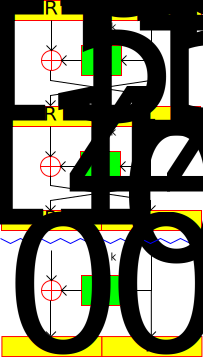
\includegraphics[width=0.8\textwidth]{out/feistel_network-decrypt.eps}
    \caption{Decryption}
    \label{fig:feistel_network_decrypt}
  \end{subfigure}
  \caption{Feistel Networks}
  \label{fig:feistel_networks}
\end{figure}
\FloatBarrier

\begin{figure}[h!]
  \centering
  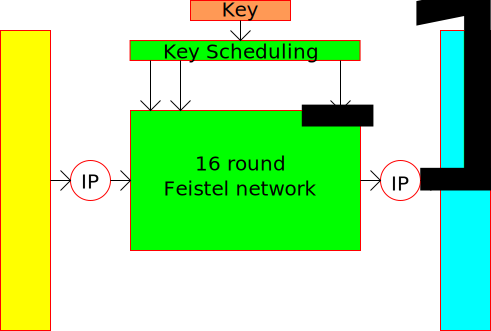
\includegraphics[width=0.6\textwidth]{out/des.eps}
  \caption{DES overview}
  \label{fig:des}
\end{figure}
\FloatBarrier

\begin{figure}[h!]
  \centering
  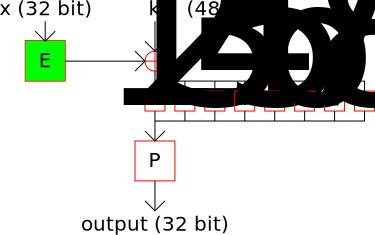
\includegraphics[width=0.6\textwidth]{out/des-function.eps}
  \caption{$F$ function}
  \label{fig:des-function}
\end{figure}
\FloatBarrier

\begin{itemize}
  \item $F$ function adds confusion and diffusion
  \item $S$ box (look up table) adds confusion
  \item $P$ box (look up table) adds diffusion
\end{itemize}

\subsubsection{Triple DES}

\begin{figure}[h!]
  \centering
  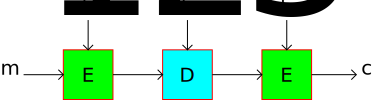
\includegraphics[width=0.6\textwidth]{out/triple-des.eps}
  \caption{Triple DES}
  \label{fig:triple-des}
\end{figure}
\FloatBarrier

\begin{itemize}
  \item Does not triple security
  \item Design is compatible with standard DES
\end{itemize}

\subsubsection{Modes of Operation}

Defines how a block cipher $E$ is applied to encrypt data.

\Para{Electronic Code Book (ECB)}

\begin{itemize}
  \item Simplest mode of operation
  \item Message split into several blocks and each block encrypted individually
  \item Deterministic
  \item Possibility of leaking data through patterns in cipher data
\end{itemize}

\begin{figure}[h!]
  \centering
  \includegraphics[width=0.8\textwidth]{out/bc-ecb.eps}
  \caption{Electronic Codebook}
  \label{fig:bc-ecb}
\end{figure}
\FloatBarrier

\Para{Cipher Block Chaining (CBC)}

\begin{itemize}
  \item Previous cipher text feeds back to next block
  \item Padding added to ensure correct block size
  \item Random initialisation vector $IV$ used to ensure non-deterministic
        output
  \item Can resynchronise if a block is lost (not if a single byte is lost)
  \item Cannot be parallelised
  \item Widely used
\end{itemize}

\begin{figure}[h!]
  \centering
  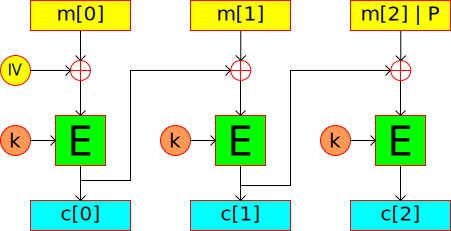
\includegraphics[width=0.8\textwidth]{out/bc-cbc.eps}
  \caption{Cipher Block Chaining}
  \label{fig:bc-cbc}
\end{figure}
\FloatBarrier

\Para{Cipher Feedback (CFB)}

\begin{itemize}
  \item Essentially a stream cipher
  \item Can resynchronise if a block is lost (not if a single byte is lost)
  \item Encryption cannot be parallelised
  \item Decryption is a single $E$ operation per block (can be parallelised)
\end{itemize}

\begin{figure}[h!]
  \centering
  \includegraphics[width=0.8\textwidth]{out/bc-cfb.eps}
  \caption{Cipher Feedback}
  \label{fig:bc-cfb}
\end{figure}
\FloatBarrier

\Para{Output Feedback (OFB)}

\begin{itemize}
  \item Essentially a stream cipher
  \item Identical encryption and decryption operations
\end{itemize}

\begin{figure}[h!]
  \centering
  \includegraphics[width=0.8\textwidth]{out/bc-ofb.eps}
  \caption{Output Feedback}
  \label{fig:bc-ofc}
\end{figure}
\FloatBarrier

\Para{Counter (CRT)}

\begin{itemize}
  \item Essentially a stream cipher
  \item Uses an incrementing counter $i$ instead of initialisation vector
  \item Identical encryption and decryption operations
  \item Both encryption and decryption can be parallelised
  \item Popular as a replacement for CBC
\end{itemize}

\begin{figure}[h!]
  \centering
  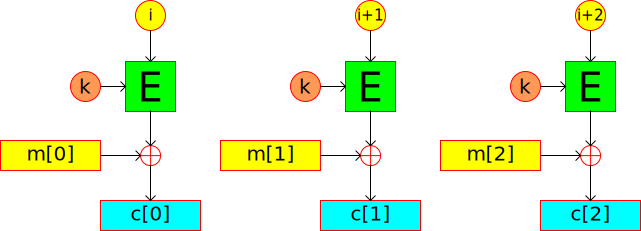
\includegraphics[width=0.8\textwidth]{out/bc-crt.eps}
  \caption{Counter}
  \label{fig:bc-crt}
\end{figure}
\FloatBarrier

\subsection{Hash Function}

\begin{itemize}
  \item Compress an arbitrary message into a fixed length output.
  \item Historically used for detecting data defects or equality
  \item Cryptographic hash used to verify integrity
\end{itemize}

\subsubsection{Random Oracle Model}

\begin{itemize}
  \item Ideal hash function
  \item Function generates a unique random hash for every new request
  \item Maintains database of existing hashes for duplicate requests
  \item No hash collisions
  \item Not practical to implement
\end{itemize}

\subsubsection{Security Requirements}

\begin{enumerate}
  \item[1]
    Pre-image resistance \\
    Given $H(m)$, cannot obtain $m$
  \item[2]
    Second pre-image resistance \\
    Given $H(m_{1})$ cannot find $m_{2}$ such that $H(m_{1}) = H(m_{2})$
  \item[3]
    Collision resistance \\
    Cannot obtain unique $m_{1}$ and $m_{2}$ such that $H(m_{1}) = H(m_{2})$
\end{enumerate}

\subsubsection{Birthday attack (collision resistance)}

Assume a hash function with $n$ bits output.

\begin{enumerate}
  \item[1] Select $2^{n/2}$ random input messages
  \item[2] Compute hash of each message
  \item[3] Look for a collision, if not found repeat until a collision occurs
\end{enumerate}

For $n$ bit security, hash output must be at least $2n$ bits long.

\subsubsection{Design considerations}

\begin{itemize}
  \item Operational mode
  \item Compression function
  \item Confusion-diffusion operations
\end{itemize}

\subsubsection{Construction: Merkle-Damgard}

\begin{itemize}
  \item Start with a fixed initialisation vector $IV$
  \item Cascade several compression functions, $f$
  \item $f$ operates over fixed length subsections of the message $m$
  \item Padding $P$ is added to ensure correct length
\end{itemize}

\begin{figure}[h!]
  \centering
  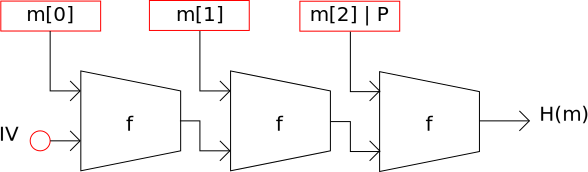
\includegraphics[width=0.8\textwidth]{out/merkle-damgard.eps}
  \caption{Merkle-Damgard construction}
  \label{fig:merkle-damgard}
\end{figure}
\FloatBarrier

Theorem is that if $f$ is collision resistant then $H$ is also collision
resistant.

\Para{Proof}

TODO

\subsubsection{Compression function: Davies-Meyer}

$E$ is a block cipher using output of previous $f$ (or $IV$ if is first block)
as message and $m[i]$ as key.

Defined as:
\[
  f(H, m) = E(m, H) \oplus H
\]

Compression:
\begin{align*}
   |input| &= |key| + |block| \\
  |output| &= |block|
\end{align*}

\begin{figure}[h!]
  \centering
  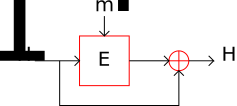
\includegraphics[width=0.4\textwidth]{out/davies-meyer.eps}
  \caption{Davies-Meyer compression function}
  \label{fig:davies-meyer}
\end{figure}
\FloatBarrier

\subsubsection{Applications}

\begin{itemize}
  \item Digital signatures
  \item Integrity checking
  \item Random number generator, random function
  \item Password masking/storage
\end{itemize}

\subsubsection{Salt}

Hashing passwords with a salt is better practice, this makes it more difficult
for an attacker to recover the plain text password.

\Para{Dictionary attack}

Given $H(password, salt)$ and $salt$ an attacker can do an exhaustive search for
all passwords and obtain the correct one.

Feasible since passwords have low entropy.

\subsection{MAC}

\begin{itemize}
  \item Used to verify integrity of a message
  \item Sender generates a tag $t$ using function $S$ and secret key $k$
  \item Recipient generates tag from message and $k$ using $S$ and compares to
        the tag sent by the sender
  \item Use of a secret key ensures the tab cannot simply be recomputed by an
        attacker
\end{itemize}

\subsubsection{Security}

Attacker can use a chosen message attack to try to obtain the key $k$.

Given a set of messages $M = \{m_{1}, m_{2}, \ldots, m_{n}\}$ and their tags $T
= \{t_{1}, t_{2}, \ldots, t_{n}\}$ such that $t_{i} \leftarrow S(k, m_{i})$.

Attacker's goal is existential forgery, i.e. producing a new message/tag pair
$(m, t) \in \{M, T\}$. In this case the attacker can successfully forge a tag
that the recipient would believe is valid.

\subsubsection{Construction 1: block cipher based}

Cipher Block Chaining (CBC) method.

\begin{figure}[h!]
  \centering
  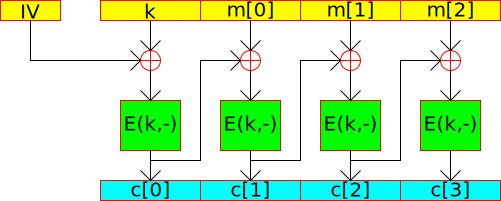
\includegraphics[width=0.8\textwidth]{out/cbc-mac.eps}
  \caption{CBC-MAC}
  \label{fig:cbc-mac}
\end{figure}
\FloatBarrier

MAC is given by $c[3]$.

\subsubsection{Construction 2: hash function based}

Cannot simply use the hash function $H(k, m)$ as an additional message block can
be added to the existing hash (see figure \ref{fig:merkle-damgard}).

\Para{HMAC}

Needs to have different secret keys to protect both the front and back of the
hash.

e.g. $H(k_{1}, H(k_{2}, m))$

In HMAC only one key is used for efficiency and two constants $O_{pad}$ and
$I_{pad}$ are used to derive $k_{1}$ and $k_{2}$.

\[
  HMAC(k, m) = H(k \oplus O_{pad} || H(k \oplus I_{pad} || m))
\]

\begin{figure}[h!]
  \centering
  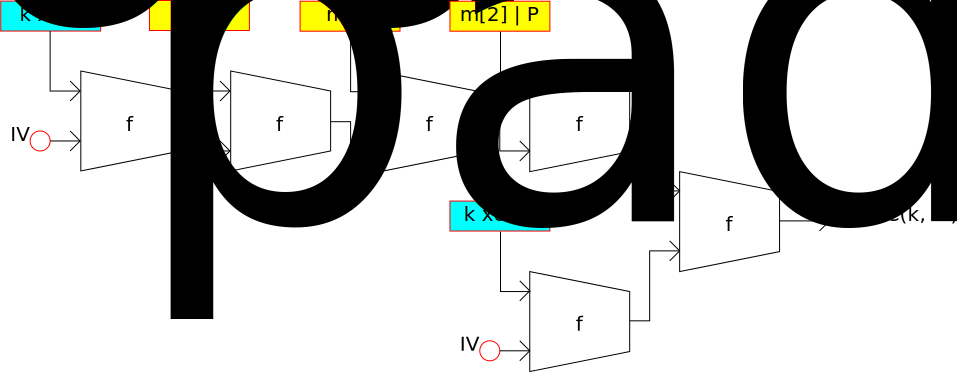
\includegraphics[width=0.9\textwidth]{out/hmac.eps}
  \caption{HMAC}
  \label{fig:hmac}
\end{figure}
\FloatBarrier

\subsubsection{Verification timing attack}

Some cryptographic libraries implement MAC verification with a byte by byte
comparison which returns false at the first incorrect byte.

By measuring the time it takes MAC verification to fail an attacker can
determine which byte of the MAC the verification failed on, therefore allowing
them to obtain the MAC by exhaustive search.

The solution is to make the verification always take the same time, the simplest
way is to perform comparison of all bytes regardless of any previous
inequalities.

\subsubsection{Authenticated encryption}

In real world applications encryption often takes place in authenticated mode,
as part of this a MAC is generated during the encryption process.

This provides both confidentiality (through the encryption) and integrity
(through the MAC).

\section{Asymmetric}

\subsection{Key Exchange}

\begin{itemize}
  \item Need to transmit a secret key on an open channel without eavesdroppers
        learning the key
  \item Too many keys to manage for each pair of participants to have their own
        key ($\mathcal{O}(n^{2})$)
  \item Ad-hoc method of key exchange is required in order to establish a secure
        communication channel between two parties
\end{itemize}

\begin{figure}[h!]
  \centering
  \includegraphics[width=0.6\textwidth]{out/key_exchange_problem.eps}
  \caption{Key Exchange Problem}
  \label{fig:key_exchange_problem}
\end{figure}
\FloatBarrier

\subsubsection{Trusted Third Party}

\begin{itemize}
  \item Only $\mathcal{O}(n)$ keys required
  \item No third party can be truly/fully trusted
\end{itemize}

\subsubsection{Merkle Puzzles}

\begin{itemize}
  \item Only secure against eavesdropping
  \item Only uses symmetric primitives
  \item Not used in real world applications
\end{itemize}

\begin{figure}[h!]
  \centering
  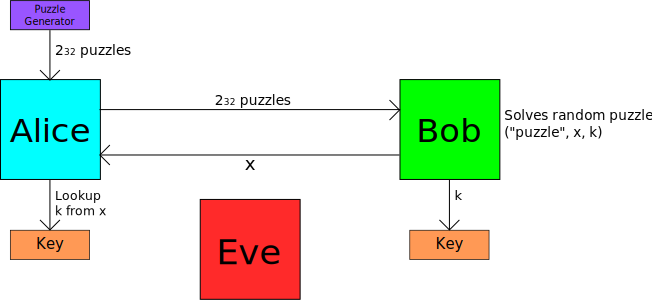
\includegraphics[width=0.8\textwidth]{out/merkle_puzzles_key_exchange.eps}
  \caption{Merkle Puzzles Key Exchange}
  \label{fig:merkle_puzzles_key_exchange}
\end{figure}
\FloatBarrier

\Para{Idea}

\begin{enumerate}
  \item[1] Alice generates a large number of puzzles (e.g. $2^{32}$) each with a
           candidate session key in the payload
  \item[2] Alice sends all the puzzles to Bob
  \item[3] Bob chooses a puzzle at random and solves it by brute force
  \item[4] Bob sends the puzzle ID back to Alice, Alice then knows which puzzle
           hence which session key Bob is using
  \item[5] Alice sends a random number $N$ to Bob, encrypted with the
           chosen session key
  \item[6] Bob replies with $N-1$ encrypted using the chosen session key
  \item[7] If the message from bob is actually $N-1$ then the key exchange was
           successful
\end{enumerate}

Choose AES key with leading zeros such that:
\[K = \{0\}^{128-l} \{0,1\}^{l}\]

Requires $2^{l}$ brute force decryption attempts to solve.

\Para{Puzzle generator}

\begin{enumerate}
  \item[1] Choose random $P \in \{0,1\}^{32}$
  \item[2] Choose random $x, k \in \{0,1\}^{128}$
  \item[3] Puzzle $P = E((\{0\}^{96}||P), "puzzle" x, k)$
\end{enumerate}

\Para{Puzzle structure}

\begin{description}
  \item[$\{0\}^{96} || P$] \hfill \\
    Random encryption key
  \item[$"puzzle" x$] \hfill \\
    Random ID
  \item[$k$] \hfill \\
    Random session key
\end{description}

\Para{Computational gap}

\begin{itemize}
  \item Workload for Alice and Bob: $\mathcal{O}(n)$, e.g. $2^{32}$
  \item Workload for Eve: $\mathcal{O}(n^{2})$, e.g. $2^{64}$
  \item Quadratic gap is best achievable for symmetric block ciphers
\end{itemize}

\subsubsection{Diffie-Hellman}

\begin{itemize}
  \item Only secure against eavesdropping
  \item Uses asymmetric primitives
\end{itemize}

\begin{figure}[h!]
  \centering
  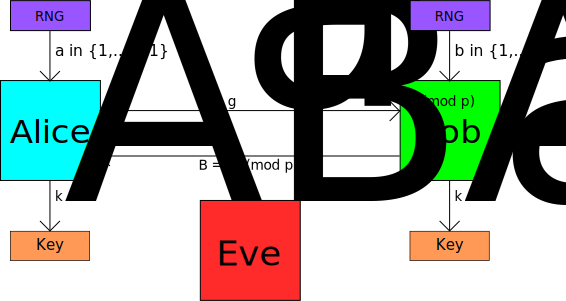
\includegraphics[width=0.6\textwidth]{out/diffie_hellman_key_exchange.eps}
  \caption{Diffe-Hellman Key Exchange}
  \label{fig:diffe_hellman_key_exchange}
\end{figure}
\FloatBarrier

\Para{Idea}

\begin{enumerate}
  \item[1] A large prime number $p$ and integer $g$ (generator of
           $(\mathbb{Z}_{p})^{*}$) are known by everyone
  \item[2] Alice chooses a random $a \in \mathbb{Z}_{p} / \{0\}$
  \item[2] Bob chooses a random $b \in \mathbb{Z}_{p} / \{0\}$
  \item[3] Alice transmits $A = g^{a} (\Mod p)$ to Bob
  \item[4] Bob transmits $B = g^{b} (\Mod p)$ to Alice
  \item[5] Alice computes session key $k_{AB} = B^{a}$
  \item[6] Bob computes session key $k_{AB} = A^{b}$
\end{enumerate}

\Para{Proof of correctness}

Proof of correctness of session keys:
\begin{align*}
  k_{AB(alice)} &= k_{AB(bob)} \\
  B^{a} &= A^{b} \\
  g^{b^{a}} &= g^{a^{b}} \\
  g^{ba} &= g^{ab} \\
  g^{ab} &= g^{ab}
\end{align*}

\Para{Difficulty}

\begin{table}[h]
  \centering
  \begin{tabular}{@{}ll@{}}
    \toprule
    Symmetric Cipher Key Size & DH/RSA Modulus Size \\
    \midrule
    80 bits                   & 1028 bits           \\
    128 bits                  & 3072 bits           \\
    \bottomrule
  \end{tabular}
  \caption{Diffie-Hellman Difficulty}
  \label{tab:diffie_hellman_difficulty}
\end{table}
\FloatBarrier

Best known algorithm to break DH/RSA is General Number Field Sieve, the expected
running time of which is $\mathcal{O}(exp(log(N)^{\frac{1}{3}}))$.

\subsubsection{Establishing a secure channel}

\begin{itemize}
  \item Messages are sent encrypted with a symmetric cipher with a MAC
  \item Avoid using same key for all ciphers and MAC generation by using key
        derivation
\end{itemize}

\begin{figure}[h!]
  \centering
  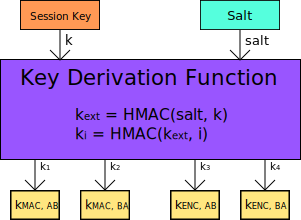
\includegraphics[width=0.6\textwidth]{out/key_derivation_function.eps}
  \caption{Key Derivation Function}
  \label{fig:key_derivation_function}
\end{figure}
\FloatBarrier

Key derivation generates different keys for cipher and MAC in both directions (4
unique keys in total) using the session key and a known salt.

\subsection{Public Key Encryption}

\subsubsection{RSA}

TODO

\subsubsection{ElGamal}

TODO

\subsection{Digital Signatures}

\subsubsection{RSA}

TODO

\subsection{Zero Knowledge Proofs}

TODO

\end{document}
